\documentclass[]{elsarticle} %review=doublespace preprint=single 5p=2 column
%%% Begin My package additions %%%%%%%%%%%%%%%%%%%
\usepackage[hyphens]{url}

  \journal{Transportation Findings} % Sets Journal name


\usepackage{lineno} % add
\providecommand{\tightlist}{%
  \setlength{\itemsep}{0pt}\setlength{\parskip}{0pt}}

\usepackage{graphicx}
\usepackage{booktabs} % book-quality tables
%%%%%%%%%%%%%%%% end my additions to header

\usepackage[T1]{fontenc}
\usepackage{lmodern}
\usepackage{amssymb,amsmath}
\usepackage{ifxetex,ifluatex}
\usepackage{fixltx2e} % provides \textsubscript
% use upquote if available, for straight quotes in verbatim environments
\IfFileExists{upquote.sty}{\usepackage{upquote}}{}
\ifnum 0\ifxetex 1\fi\ifluatex 1\fi=0 % if pdftex
  \usepackage[utf8]{inputenc}
\else % if luatex or xelatex
  \usepackage{fontspec}
  \ifxetex
    \usepackage{xltxtra,xunicode}
  \fi
  \defaultfontfeatures{Mapping=tex-text,Scale=MatchLowercase}
  \newcommand{\euro}{€}
\fi
% use microtype if available
\IfFileExists{microtype.sty}{\usepackage{microtype}}{}
\bibliographystyle{elsarticle-harv}
\usepackage{graphicx}
% We will generate all images so they have a width \maxwidth. This means
% that they will get their normal width if they fit onto the page, but
% are scaled down if they would overflow the margins.
\makeatletter
\def\maxwidth{\ifdim\Gin@nat@width>\linewidth\linewidth
\else\Gin@nat@width\fi}
\makeatother
\let\Oldincludegraphics\includegraphics
\renewcommand{\includegraphics}[1]{\Oldincludegraphics[width=\maxwidth]{#1}}
\ifxetex
  \usepackage[setpagesize=false, % page size defined by xetex
              unicode=false, % unicode breaks when used with xetex
              xetex]{hyperref}
\else
  \usepackage[unicode=true]{hyperref}
\fi
\hypersetup{breaklinks=true,
            bookmarks=true,
            pdfauthor={},
            pdftitle={Using Google Community Mobility Reports to investigate the growth of COVID-19 in the United States},
            colorlinks=false,
            urlcolor=blue,
            linkcolor=magenta,
            pdfborder={0 0 0}}
\urlstyle{same}  % don't use monospace font for urls

\setcounter{secnumdepth}{0}
% Pandoc toggle for numbering sections (defaults to be off)
\setcounter{secnumdepth}{0}


% Pandoc header
\usepackage{booktabs}
\usepackage{longtable}
\usepackage{array}
\usepackage{multirow}
\usepackage{wrapfig}
\usepackage{float}
\usepackage{colortbl}
\usepackage{pdflscape}
\usepackage{tabu}
\usepackage{threeparttable}
\usepackage{threeparttablex}
\usepackage[normalem]{ulem}
\usepackage{makecell}
\usepackage{xcolor}



\begin{document}
\begin{frontmatter}

  \title{Using Google Community Mobility Reports to investigate the growth of
COVID-19 in the United States}
    \author[McMaster University]{Antonio Paez\corref{1}}
   \ead{paezha@mcmaster.ca} 
      \address[McMaster University]{School of Geography and Earth Sciences, McMaster University, Hamilton,
ON, L8S 4K1, Canada}
      \cortext[1]{Corresponding Author}
  
  \begin{abstract}
  In 2020 Google released a set of Community Mobility Reports (GCMR).
  These reports are based on the company's location-tracking capabilities
  and measure changes in mobility with respect to a baseline. This novel
  source of data offers an opportunity to investigate the way mobility
  potentially correlates with transmission of COVID-19. Using data from
  the New York Times on COVID-19 cases and GCMR, this paper presents an
  analysis of mobility levels and new daily reported cases of COVID-19 by
  state in the US. The results provide insights about the utility and
  interpretability of GCMR for COVID-19 research and decision-making.
  \end{abstract}
  
 \end{frontmatter}

\hypertarget{research-questions-and-hypotheses}{%
\section{Research Questions and
Hypotheses}\label{research-questions-and-hypotheses}}

The main policy tool to control the spread of the COVID-19 pandemic has
been stay-at-home orders. Concurrently, numerous efforts exist to track
the progress and the impact of the pandemic, and new sources of data
include the recently-released Google Community Mobility Reports
(GCMR)\footnote{https://www.google.com/covid19/mobility/}, as well as
The New York Times repository of COVID-19
data\footnote{https://github.com/nytimes/covid-19-data}. These two open
data sets offer novel opportunities to investigate in quasi-real time
the relationship between mobility patterns and transmission of COVID-19.

This paper investigates the potential of Google Community Mobility
Reports to asses the impact of mobility on COVID-19. The following
questions are posed:

\begin{itemize}
\tightlist
\item
  Do changes in mobility according to GCMR correlate with the
  transmission of COVID-19?
\item
  And if so, what do we learn about mobility and the spread of the
  disease?
\end{itemize}

The source document for this paper is an \texttt{R} markdown document
available from the following repository:

https://github.com/paezha/Google-Mobility-Reports-and-COVID-19-US

\hypertarget{methods-and-data}{%
\section{Methods and Data}\label{methods-and-data}}

GCMR use aggregated and anonymized data to chart changes in mobility
with respect to different classes of places, namely retail and
recreation, groceries and pharmacies, parks, transit stations,
workplaces, and residential. Mobility indicators for each of these
places are reported as percentage changes from a baseline level, which
corresponds to the median value of mobility of identical days of the
week during the period between January 3 and Feb 6, 2020. Covid-19 data
is compiled by The New York Times based on reports from state and local
health agencies.

For analysis, all mobility indicators are centered so that the value of
1 is the base mobility, and a 0.01 deviation corresponds to a 1\%
change. The incubation time of the disease has been estimated to be
between 2 and 12 days (95\% interval) by Lauer et al.~(2020). Given
this, it is to be expected that any changes in mobility will have a
lagged effect on the discovery of new cases. For this reason, lagged
moving averages of the mobility indicators are calculated. Furthermore,
it is possible that mobility and reports of new cases of COVID-19 are
endogenous, if the public adjust their mobility according to reports of
the incidence. Therefore, in addition to being consistent with an
incubation period, use of lagged indicators also helps to break this
potential endogeneity.

\begin{table}[!h]

\caption{\label{tab:descriptive-statistics}\label{tab:descriptive-statistics}Descriptive statistics of the data set}
\centering
\resizebox{\linewidth}{!}{
\begin{tabular}[t]{llllll}
\toprule
Variable & Definition & min & median & max & sd\\
\midrule
\rowcolor{gray!6}  New Cases & New Daily Cases of COVID-19 & 0 & 77.5 & 12126 & 1059.81\\
date & Date & 2020-02-27 & 2020-04-01 & 2020-04-26 & \\
\rowcolor{gray!6}  retail & Retail and Recreation & 0.34 & 0.66 & 1.16 & 0.22\\
groceries & Groceries and Pharmacies & 0.66 & 0.95 & 1.26 & 0.13\\
\rowcolor{gray!6}  parks & Parks & 0.36 & 1.15 & 1.8 & 0.24\\
\addlinespace
transit & Transit Stations & 0.24 & 0.73 & 1.14 & 0.24\\
\rowcolor{gray!6}  work & Workplaces & 0.34 & 0.65 & 1.07 & 0.2\\
residential & Residential & 0.97 & 1.14 & 1.27 & 0.08\\
\bottomrule
\multicolumn{6}{l}{\textit{Note: }}\\
\multicolumn{6}{l}{All mobility indicators are lagged 11-day moving averages}\\
\end{tabular}}
\end{table}

The lagged indicators are calculated as the mean of the mobility
indicator using the values from date-minus-12-days to date-minus-2-days.
Furthermore, using the cumulative number of reported COVID-19 cases, the
total number of new daily cases is calculated. This variable
(log-transformed after adding a small constant) is paired to the
corresponding lagged moving average of the mobility indicators. The
log-transformation is useful to avoid negative values of daily new cases
when making predictions. Analysis is based on correlation analysis,
multivariate regression, and data visualization. Table
\ref{tab:descriptive-statistics} shows the descriptive statistics of the
data set. Temporal coverage is from February 27 to April 26, 2020. The
maximum number of new daily cases during this period is 12,126.

\hypertarget{findings}{%
\section{Findings}\label{findings}}

Table \ref{tab:correlation-analysis} shows that the mobility indicators
are highly correlated with each other. This is not surprising: it is
well-known that mobility involves time-use trade-offs: the more there is
of one kind of mobility, the less time there is available for any other.
That said, the strongest correlation with the outcome of interest is for
residential-based mobility. To avoid multicollinearity, parks-related
mobility is selected as a covariate since it has the lowest correlation
with residential-based mobility.

\begin{table}[!h]

\caption{\label{tab:check-correlations}\label{tab:correlation-analysis}Simple correlation between log(New Cases) and the mobility indicators}
\centering
\resizebox{\linewidth}{!}{
\begin{tabular}[t]{lrrrrrrr}
\toprule
  & log\_new\_cases & retail & groceries & parks & transit & work & residential\\
\midrule
\rowcolor{gray!6}  log\_new\_cases & 1.00 & -0.68 & -0.47 & -0.30 & -0.68 & -0.69 & 0.71\\
retail & -0.68 & 1.00 & 0.86 & 0.44 & 0.93 & 0.98 & -0.98\\
\rowcolor{gray!6}  groceries & -0.47 & 0.86 & 1.00 & 0.46 & 0.87 & 0.87 & -0.86\\
parks & -0.30 & 0.44 & 0.46 & 1.00 & 0.52 & 0.44 & -0.45\\
\rowcolor{gray!6}  transit & -0.68 & 0.93 & 0.87 & 0.52 & 1.00 & 0.94 & -0.95\\
\addlinespace
work & -0.69 & 0.98 & 0.87 & 0.44 & 0.94 & 1.00 & -0.99\\
\rowcolor{gray!6}  residential & 0.71 & -0.98 & -0.86 & -0.45 & -0.95 & -0.99 & 1.00\\
\bottomrule
\multicolumn{8}{l}{\textit{Note: }}\\
\multicolumn{8}{l}{All mobility indicators are lagged 11-day moving averages}\\
\end{tabular}}
\end{table}

A regression model uses the log of new daily cases as the dependent
variable. The covariates are parks- and residential-related mobility,
which enter the regression in the form of a second order polynomial
expansion. In addition, the date is introduced to account for the
temporal trend of the pandemic. Finally, an indicator variable for the
state of New York and an interaction with the date are used to
distinguish the unusually high incidence of the disease there. The
results appear in Table \ref{tab:model-results}. The model provides a
good fit to the data and all variables reported are significant at
\(p<0.05\) or better.

There is an overall temporal trend that indicates a growing number of
cases over time, but at a decreasing rate (see negative sign of
date\^{}2). New York has on average more new daily cases than the rest
of the states, but this has also declined over time (see negative sign
of NY x date). Visualization is the most effective way to understand the
trend according to the mobility indicators and date. Figure
\ref{fig:prediction-plots} shows the prediction surfaces on three
different dates: March 21, when the first states began implementing
stay-at-home orders; April 5, fifteen days later; and April 20, fifteen
more days later, and at a time when some states are considering relaxing
stay-at-home orders. On March 21 there were still only minor departures
from baseline mobility (recall that these are temporally lagged); the
prediction surface at this point is relatively flat. This changes by
April 5, when large increases in residential-based mobility are seen,
along with greater variations in parks-based mobility. The prediction
surface indicates an expectation of a greater number of new daily cases
as both classes of mobility increase. On the last date examined, April
20, the trend becomes more steep for park-based mobility, even as this
indicator continues to display large variations from the baseline in
both directions. In general, higher levels of mobility tend to be
associates with a higher number of new daily cases.

\begin{table}[!h]

\caption{\label{tab:model-results}\label{tab:model-results}Results of estimating regression model. Dependent variable is log(New Cases + 0.0001).}
\centering
\begin{tabular}[t]{lcc}
\toprule
Variable & Coefficient Estimate & p-value\\
\midrule
\rowcolor{gray!6}  date & 7.9619 & <0.0001\\
date\textasciicircum{}2 & -0.0411 & <0.0001\\
\rowcolor{gray!6}  parks\textasciicircum{}2 & 1.4017 & 0.0251\\
parks & -37.2492 & <0.0001\\
\rowcolor{gray!6}  parks x residential & 39.0902 & <0.0001\\
\addlinespace
residential & -286.7568 & <0.0001\\
\rowcolor{gray!6}  residential\textasciicircum{}2 & 249.9901 & <0.0001\\
parks x date & -0.1412 & <0.0001\\
\rowcolor{gray!6}  residential x date & -6.9180 & <0.0001\\
residential x date\textasciicircum{}2 & 0.0365 & <0.0001\\
\addlinespace
\rowcolor{gray!6}  NY & 6.9864 & <0.0001\\
NY x date & -0.0557 & 0.0022\\
\bottomrule
\multicolumn{3}{l}{\textit{Note: }}\\
\multicolumn{3}{l}{Coefficient of Determination $R^2$= 0.821}\\
\multicolumn{3}{l}{Adjusted Coefficient of Determination $R^2$= 0.82}\\
\multicolumn{3}{l}{Standard Error $\sigma$= 2.102}\\
\end{tabular}
\end{table}

\begin{figure}
\centering
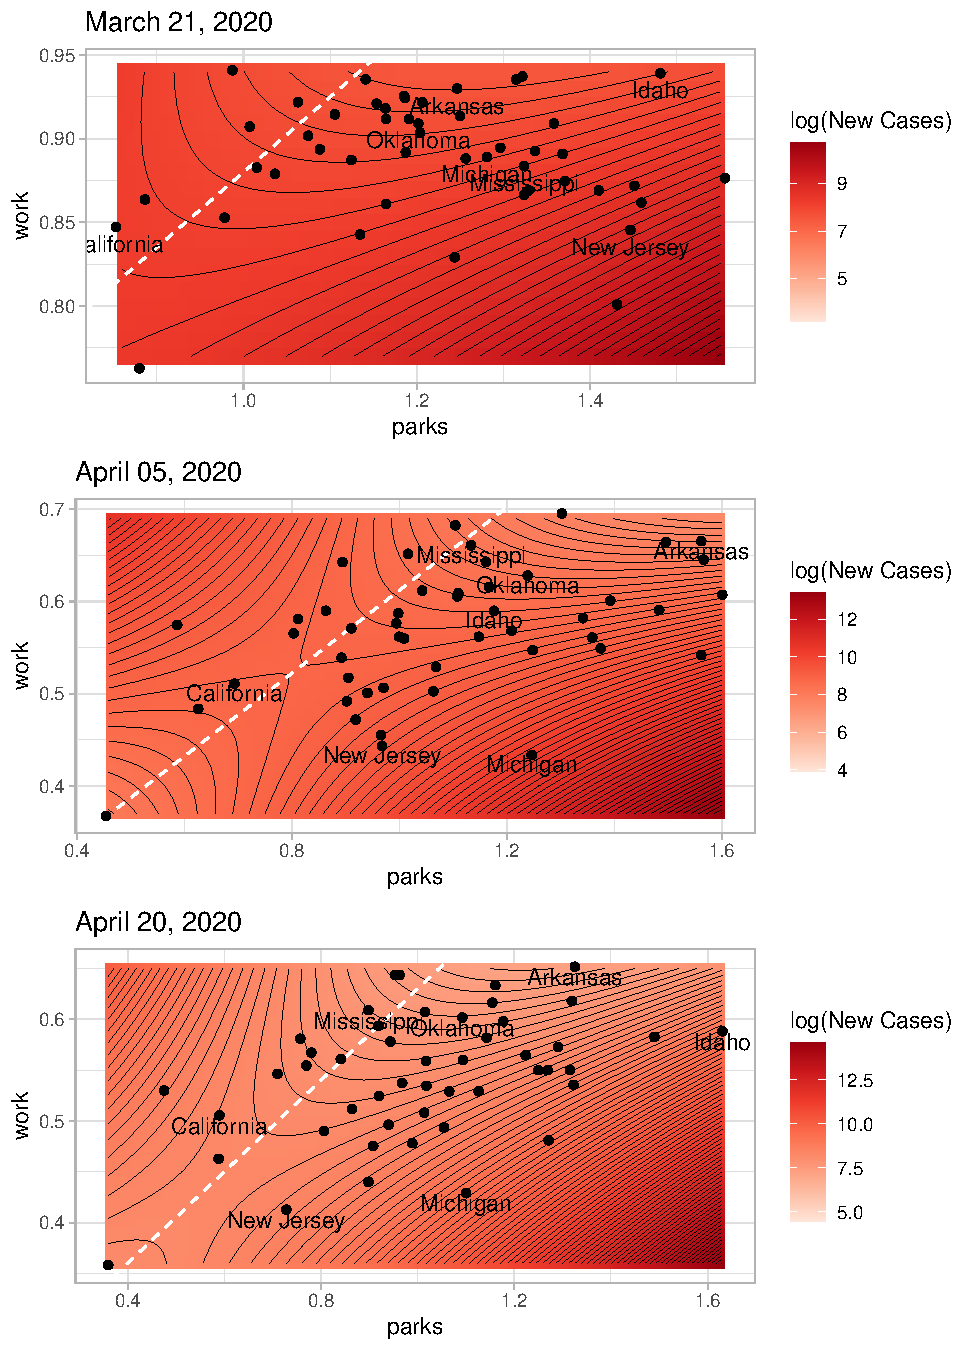
\includegraphics{Covid-19-Google-CMR-US_files/figure-latex/prediction-plots-1.pdf}
\caption{\label{fig:prediction-plots}Prediction surfaces at three points
during the pandemic according to the model; the dots are scatterplots of
the park- and residential-mobility indicators of the states on that
date.}
\end{figure}

The results suggest the potential of GCMR to investigate the spread of
COVID-19, but also point at some limitations. The baseline level is not
defined in a metric that is amenable to policy development (Google
defines ``mobility'' as an aggregated score of visits and length of stay
at places.) For example, it is not clear precisely what is residential
mobility: is it visits with friends and relatives, or mobility in the
vicinity of the place of residency? Without a clearer understanding of
these variables, their use can suggest trends, but their potential for
applied policy analysis appears to be more limited.

\hypertarget{references}{%
\section*{References}\label{references}}
\addcontentsline{toc}{section}{References}

\hypertarget{refs}{}
\leavevmode\hypertarget{ref-Lauer2020incubation}{}%
Lauer, S.A., Grantz, K.H., Bi, Q., Jones, F.K., Zheng, Q., Meredith,
H.R., Azman, A.S., Reich, N.G., Lessler, J., 2020. The incubation period
of coronavirus disease 2019 (covid-19) from publicly reported confirmed
cases: Estimation and application. Annals of Internal Medicine.
doi:\href{https://doi.org/10.7326/m20-0504}{10.7326/m20-0504}


\end{document}


